%%%%%%%%%%%%%%%%%%%%%%%%%%%%%%%%%%%%%%%%%
% Beamer Presentation
% LaTeX Template
% Version 1.0 (10/11/12)
%
% This template has been downloaded from:
% http://www.LaTeXTemplates.com
%
% License:
% CC BY-NC-SA 3.0 (http://creativecommons.org/licenses/by-nc-sa/3.0/)
%
%%%%%%%%%%%%%%%%%%%%%%%%%%%%%%%%%%%%%%%%%

%----------------------------------------------------------------------------------------
%	PACKAGES AND THEMES
%----------------------------------------------------------------------------------------

%\documentclass[UTF8,aspectratio=169,14pt]{ctexbeamer}
\documentclass[UTF8,aspectratio=169]{ctexbeamer}
\usepackage{hyperref}
\hypersetup{
	colorlinks=true,
	linkcolor=red,
	anchorcolor=blue,
	citecolor=green
}

\mode<presentation> {
	
	% The Beamer class comes with a number of default slide themes
	% which change the colors and layouts of slides. Below this is a list
	% of all the themes, uncomment each in turn to see what they look like.
	
	%\usetheme{default}
	%\usetheme{AnnArbor}
	%\usetheme{Antibes}
	%\usetheme{Bergen}
	%\usetheme{Berkeley}
	%\usetheme{Berlin}
	%\usetheme{Boadilla}
	%\usetheme{CambridgeUS}
	%\usetheme{Copenhagen}
	%\usetheme{Darmstadt}
	%\usetheme{Dresden}
	%\usetheme{Frankfurt}
	%\usetheme{Goettingen}
	%\usetheme{Hannover}
	%\usetheme{Ilmenau}
	%\usetheme{JuanLesPins}
	%\usetheme{Luebeck}
	\usetheme{Madrid}
	%\usetheme{Malmoe}
	%\usetheme{Marburg}
	%\usetheme{Montpellier}
	%\usetheme{PaloAlto}
	%\usetheme{Pittsburgh}
	%\usetheme{Rochester}
	%\usetheme{Singapore}
	%\usetheme{Szeged}
	%\usetheme{Warsaw}
	
	% As well as themes, the Beamer class has a number of color themes
	% for any slide theme. Uncomment each of these in turn to see how it
	% changes the colors of your current slide theme.
	
	%\usecolortheme{albatross}
	%\usecolortheme{beaver}
	%\usecolortheme{beetle}
	%\usecolortheme{crane}
	%\usecolortheme{dolphin}
	%\usecolortheme{dove}
	%\usecolortheme{fly}
	%\usecolortheme{lily}
	%\usecolortheme{orchid}
	%\usecolortheme{rose}
	%\usecolortheme{seagull}
	%\usecolortheme{seahorse}
	%\usecolortheme{whale}
	%\usecolortheme{wolverine}
	
	%\setbeamertemplate{footline} % To remove the footer line in all slides uncomment this line
	%\setbeamertemplate{footline}[page number] % To replace the footer line in all slides with a simple slide count uncomment this line
	
	%\setbeamertemplate{navigation symbols}{} % To remove the navigation symbols from the bottom of all slides uncomment this line
}

\usepackage{graphicx} % Allows including images
\graphicspath{{./figs/}}
\usepackage{booktabs} % Allows the use of \toprule, \midrule and \bottomrule in tables
\usepackage{longtable}
\usepackage{listings}
\usepackage{xcolor}
\lstset{numbers=left, %设置行号位置
	numberstyle=\tiny, %设置行号大小
	keywordstyle=\color{blue}, %设置关键字颜色
	commentstyle=\color[cmyk]{1,0,1,0}, %设置注释颜色
	frame=single, %设置边框格式
	escapeinside=``, %逃逸字符(1左面的键),用于显示中文
	%breaklines, %自动折行
	extendedchars=false, %解决代码跨页时,章节标题,页眉等汉字不显示的问题
	xleftmargin=2em,xrightmargin=2em, aboveskip=1em, %设置边距
	tabsize=4, %设置tab空格数
	showspaces=false %不显示空格
}
% Fonts
% \usepackage{libertine}
% \setmonofont{Courier}
\setCJKsansfont[ItalicFont=Noto Serif CJK SC Black, BoldFont=Noto Sans CJK SC Black]{Noto Sans CJK SC}
\setmainfont[Ligatures={Common,TeX}]{Linux  Libertine O}
\setmonofont[SmallCapsFont={Latin Modern Mono Caps}]{Latin Modern Mono Light}
\setsansfont{Linux Biolinum O}

\logo{
\includegraphics[width=0.55cm,height=0.55cm]{../../thcs-logo.png}}
%\def\imagepath{./resources/graphics}
%\usepackage[imagepath=\imagepath]{ditaa}
%\graphicspath{ {\imagepath/} }


%\usepackage{pgfpages}
%\setbeameroption{show notes on second screen}
%%----------------------------------------------------------------------------------------
%	TITLE PAGE
%----------------------------------------------------------------------------------------

\title[第1讲]{第1讲 :操作系统概述} % The short title appears at the bottom of every slide, the full title is only on the title page
\subtitle{第一节:课程概述}
\author{向勇、陈渝} % Your name
\institute[清华大学] % Your institution as it will appear on the bottom of every slide, may be shorthand to save space
{
	清华大学计算机系 \\ % Your institution for the title page
	\medskip
	\textit{xyong,yuchen@tsinghua.edu.cn} % Your email address
}
\date{\today} % Date, can be changed to a custom date


\begin{document}

\begin{frame}
\titlepage % Print the title page as the first slide
\end{frame}

%\begin{frame}
%\frametitle{提纲} % Table of contents slide, comment this block out to remove it
%\tableofcontents % Throughout your presentation, if you choose to use \section{} and \subsection{} commands, these will automatically be printed on this slide as an overview of your presentation
%\end{frame}
%
%%----------------------------------------------------------------------------------------
%%	PRESENTATION SLIDES
%%----------------------------------------------------------------------------------------
%
%%------------------------------------------------
%\section{第一节:课程概述} % Sections can be created in order to organize your presentation into discrete blocks, all sections and subsections are automatically printed in the table of contents as an overview of the talk
%%------------------------------------------------

%\begin{frame}[fragile]
%	\frametitle{课程信息}
%	test
%%\begin{verbatim}
%%\begin{ditaa}{ditaa caption example}{ditaaexample}
%%+--------+   +-------+    +-------+
%%|        | --+ ditaa +--> |       |
%%|  Text  |   +-------+    |diagram|
%%|Document|   |!magic!|    |       |
%%|     {d}|   |       |    |       |
%%+---+----+   +-------+    +-------+
%%:                         ^
%%|       Lots of work      |
%%+-------------------------+
%%\end{ditaa}
%%​\end{verbatim}
%
%\end{frame}
%----------------------------------------------
\begin{frame}[plain]	
	\frametitle{}

	
\end{frame}
%----------------------------------------------
\begin{frame}[plain]	
	\frametitle{}
	
\begin{itemize}\Large
	\item Apple

\end{itemize}

\centering
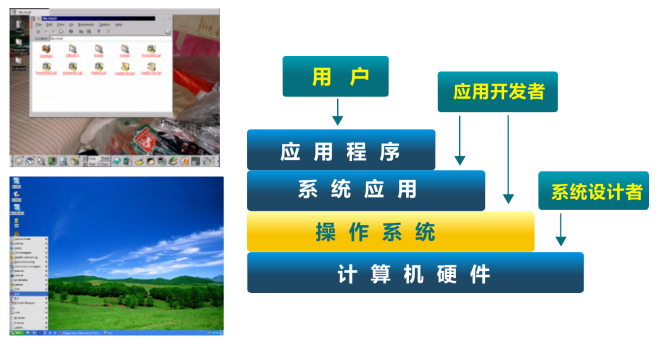
\includegraphics[width=0.8\textwidth]{os-position}
		
\end{frame}

%----------------------------------------------
\begin{frame}[plain]	
	\frametitle{}
	
	\begin{itemize}\Large
		\item Apple
		\begin{itemize}\large
			\item RedApple
			
		\end{itemize}
	\end{itemize}
	
	
\end{frame}
%----------------------------------------------
\begin{frame}[plain]	
	\frametitle{}

\begin{itemize}
	\item Apple
	\begin{itemize}
		\item RedApple
		
	\end{itemize}
\end{itemize}
	
	
\end{frame}

%----------------------------------------------
\begin{frame}[plain]	
	\frametitle{}

\begin{itemize}
	\item Apple
	

\end{itemize}	
	
\end{frame}

%----------------------------------------------
\begin{frame}[plain]	
	\frametitle{}
	
	
\end{frame}

%----------------------------------------------
\begin{frame}[t]
	\frametitle{ }
	\begin{columns}[t]
		\begin{column}{.5\textwidth}

		\begin{itemize}\Large
			\item Apple
			\begin{itemize}\large
				\item RedApple
				
			\end{itemize}
		\end{itemize}

		\end{column}
	
		\begin{column}{.5\textwidth}

		\begin{itemize}\Large
			\item Apple
			\begin{itemize}\large
				\item BlueApple
				
			\end{itemize}
		\end{itemize}
		
		\end{column}
	\end{columns}
\end{frame}

%----------------------------------------------
\begin{frame}[t]
	\frametitle{ }
	\begin{columns}[t]
		\begin{column}{.5\textwidth}
			
			\begin{itemize}\Large
				\item Apple
				\begin{itemize}\large
					\item RedApple
					
				\end{itemize}
			\end{itemize}
			
		\end{column}
		
		\begin{column}{.5\textwidth}
			
		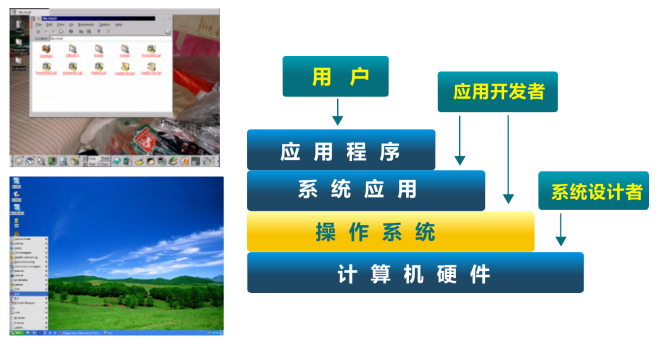
\includegraphics[width=0.6\textwidth]{os-position}
			
		\end{column}
	\end{columns}
\end{frame}

%----------------------------------------------
\begin{frame}[plain]	
	\frametitle{}
	
	
\end{frame}
\begin{frame}[plain]
	
	\frametitle{操作系统定义}
	
	\begin{flushleft} %左对齐
		Answer: rely on CPU to trap sensitive instructions and hand off to VMM
	\end{flushleft}


	\begin{flushright} %右对齐
	Answer: rely on CPU to trap sensitive instructions and hand off to VMM
	\end{flushright}


	没有公认的精确定义 \pause
	
	\begin{block}{操作系统定义}
		操作系统是管理硬件资源、控制程序运行、改善人机界面和为应用软件提供支持的一种系统软件。[计算机百科全书]
	\end{block} \pause
	
	
	\begin{figure}
		\centering
		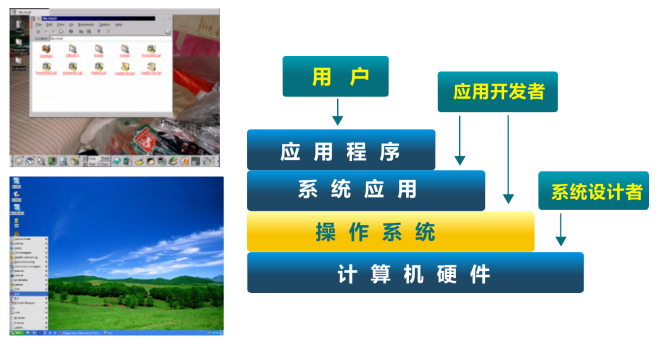
\includegraphics[width=0.5\linewidth]{os-position}
		\caption{承上启下的操作系统}
	\end{figure}
	
\end{frame}

\begin{frame}
	\frametitle{基础实验}
	\framesubtitle{rCore实验:基于RISC-V用rust写教学操作系统} \pause

	\begin{columns}

		\begin{column}{0.5\textwidth}
			\begin{itemize}
				\item 第一章:独立式可执行程序
			\end{itemize}
		\end{column}
		
		\begin{column}{0.5\textwidth}
			\begin{itemize}
				\item 第六章:内核线程
			\end{itemize}
		\end{column}
		
	\end{columns}

\end{frame}


\begin{frame}<1-2,4->
	This is slide number \only<1->{1}\only<2>{2}\only<3>{3}%
	\only<4>{4}\only<5>{5}.
\end{frame}

\begin{frame}

\begin{itemize}[<+->]
	\item Apple
	\item<.-> Peach
	\item Plum
	\item Orange
\end{itemize}
\end{frame}


\begin{itemize}[<+->]
	\item This is \alert<.>{important}.
	\item We want to \alert<.>{highlight} this and \alert<.>{this}.
	\item What is the \alert<.>{matrix}?
\end{itemize}



\begin{frame}[fragile]
	\frametitle{An Algorithm For Finding Primes Numbers.}
	\begin{verbatim}
	int main (void)
	{
	std::vector<bool> is_prime (100, true);
	for (int i = 2; i < 100; i++)
	if (is_prime[i])
	{
	std::cout << i << " ";
	for (int j = i; j < 100; is_prime [j] = false, j+=i);
	}
	return 0;
	}
	\end{verbatim}
	\begin{uncoverenv}<2>
		Note the use of \verb|std::|.
	\end{uncoverenv}
\end{frame}

\begin{frame}[fragile]
	\frametitle{An Algorithm For Finding Primes Numbers.}
	\begin{semiverbatim}
		\uncover<1->{\alert<0>{int main (void)}}
		\uncover<1->{\alert<0>{\{}}
		\uncover<1->{\alert<1>{
				\alert<4>{std::}vector<bool> is_prime (100, true);}}
		\uncover<1->{\alert<1>{
				for (int i = 2; i < 100; i++)}}
		\uncover<2->{\alert<2>{
				if (is_prime[i])}}
		\uncover<2->{\alert<0>{
				\{}}
		\uncover<3->{\alert<3>{
				\alert<4>{std::}cout << i << " ";}}
		\uncover<3->{\alert<3>{
				for (int j = i; j < 100;}}
		\uncover<3->{\alert<3>{
				is_prime [j] = false, j+=i);}}
		\uncover<2->{\alert<0>{
				\}}}
		\uncover<1->{\alert<0>{
				return 0;}}
		\uncover<1->{\alert<0>{\}}}
	\end{semiverbatim}
	\visible<4->{Note the use of \alert{\texttt{std::}}.}
\end{frame}



\begin{frame}
	\frametitle{What's Still To Do?}
	\begin{columns}
\column{.5\textwidth}
\begin{block}{Answered Questions}
	How many primes are there?
\end{block}
\column{.5\textwidth}
\begin{block}{Open Questions}
	Is every even number the sum of two primes?
\end{block}
\end{columns}
\end{frame}



\begin{frame}
	\frametitle{What's Still To Do?}
	\begin{block}{Answered Questions}
		How many primes are there?
	\end{block}
	\begin{block}{Open Questions}
		Is every even number the sum of two primes?
	\end{block}
\end{frame}


\begin{frame}
	\frametitle{What Are Prime Numbers?}
	\begin{definition}
		A \alert{prime number} is a number that has exactly two divisors.
	\end{definition}
\end{frame}



\begin{frame}
	\frametitle{课程信息}
	
	\begin{itemize}[<+->]
		\item First point.
		\item[<.->] Second point.
		\item Third point.
	\end{itemize}
	
	
	
\end{frame}

\begin{frame}
	\frametitle{课程信息}
	
\begin{itemize}
	\item<1-| alert@1> First point.
	\item<2-| alert@2> Second point.
	\item<3-| alert@3> Third point.
\end{itemize}
	
	
\end{frame}

	
\begin{frame}
	\frametitle{课程信息}
	\begin{itemize}
		\item 主讲教师:向勇、陈渝
%		\pause

		\item 助教: 
\begin{itemize}
		\item<3-> 王润基、贾越凯、戴臻旸、刘丰源

		\item<3-> 吴一凡、潘庆霖、张译仁、陈嘉杰
	\end{itemize}
	\end{itemize}

\begin{itemize}
	\item<1-> First point.
	\item<2-> Second point.
	\item<3-> Third point.
\end{itemize}


\end{frame}

\begin{frame}

\frametitle{预备知识}

\begin{itemize}

\item 程序设计语言(汇编、C和Rust)
  \begin{itemize}
    \item :( 不是开发应用程序
    \item :) 而是开发系统程序
    \pause
  \end{itemize}
\item 数据结构
  \begin{itemize}
    \item :) 理解基本数据结构即可 
  \end{itemize}
\pause
\item 计算机组成原理
  \begin{itemize}
    \item :( 康总的x86/mips原理 
    \item  :)  \href{http://crva.ict.ac.cn/documents/RISC-V-Reader-Chinese-v2p1.pdf}{Patterson的RISC-V原理}
  \end{itemize}
\pause
\item 编译原理
  \begin{itemize}
    \item :) 没学过影响不大  
    \item :( 但还是要了解高级语言<-->RISC-V汇编语言

  \end{itemize}

\end{itemize}

\end{frame}

\begin{frame}
	\frametitle{课程信息}
	\begin{itemize}
		\item \href{http://os.cs.tsinghua.edu.cn/oscourse/OS2020spring}{课程\textbf{WIKI}}
		\begin{itemize}
		\item 所有课程信息的入口,也是最新课程信息的官方发布网站
	    \end{itemize}
		\pause
		\item 课程视频
		\begin{itemize}
    		\item \href{https://next.xuetangx.com/}{学堂在线}:操作系统(RISC-V)
    	\end{itemize}
		\pause
    	\item 作业
    	\begin{itemize}
    	    \item \href{http://learn.tsinghua.edu.cn/f/wlxt/index/course/teacher/course?wlkcid=2019-2020-2140259621}{网络学堂 -- 向老师}		
		    \item \href{http://learn.tsinghua.edu.cn/f/wlxt/index/course/teacher/course?wlkcid=2019-2020-2140259622}{网络学堂 -- 陈老师}
    	\end{itemize}
		\pause
    	\item 实验楼的在线实验环境
    	\begin{itemize}
		    \item \href{https://www.shiyanlou.com/courses/221}{ucore os在线实验环境}
		    \item \href{https://www.shiyanlou.com/courses/1481}{rcore os在线实验环境}
		\end{itemize}
		\item 讨论区
		\begin{itemize}
		    \item \href{https://piazza.com/tsinghua.edu.cn/spring2015/30240243x/home}{Piazza交流论坛}
		    \item 微信:OS2020
		\end{itemize}
	\end{itemize}
\end{frame}

%----------------------------------------------------------------------------------------

\end{document}
